\subsection{Invisible Z estimation}
\label{subsec:zinv}
The invisible Z background is estimated using a $Z(\ell\ell)$ plus $\gamma$ control region.
The method relies on the fact that for $\gamma Z(\nu\nu)$ events, the \ptmiss is
roughly equal to the transverse momentum of the Z boson.  There is also a small
contribution from limited resolution
of other objects in the event -- primarily jets; this effect of finite resolution
means that $p_{T,Z(\ell\ell)}$ cannot be used directly as a proxy for \ptmiss.   

The $Z(\ell\ell)$ plus $\gamma$ events are required to have one high-\pt photon and two oppositely 
charged, same flavor leptons (e, $\mu$) whose invariant mass is consistent with 
the Z mass, $80<m_{\ell\ell}<100~\gev$.  For the purposes of computing event level
kinematic variables, the effect of leptons is removed.  For \ST, \nj, \nb, and $\dphi$
jets which are matched, $\Delta R<0.3$, to the charged leptons are ignored.  For \ptmiss
the reconstructed transverse momentum of the Z candidate is added to the \ptmiss vector.
This cleaning procedure allow for finite jet resolution to smear the $p_{T,Z(\ell\ell)}$
and provide a consistent way of modeling the kinematics of neutrino decays.  The kinematic 
selections are then the same as the signal region, but using these ``cleaned'' variables.  

$Z(\ell\ell)$ plus $\gamma$ events have one primary difference with respect to $Z(\nu\nu)+\gamma$
events;  the former can result from the photon being radiated by charged leptons from the
Z boson decay.  This effect is small for our phase space, $p_{T,Z(\ell\ell)}$~\ptmiss$>100~\gev$ and 
$\ptg>100~\gev$.  However, these events will typically produce a photon which is
roughly colinear with one of the charged leptons in the event.  We require that the angle 
between any electron or muon and the photon be $\Delta R(e/\mu,\gamma)>0.2$. We also 
require the invariant mass of di-lepton pair to be in the range $80-100\ \gev$ which further supresses 
the photon radiation from lepton.

The triggers for the $\gamma$-DY control region are the same as the signal region
triggers.

Because of the low statistics for Z($\ell\ell$)+$\gamma$ events, the \ptmiss shape will be taken directly from MC.  
The overall event yield will be measured by scaling the $Z(\nu\nu)+\gamma$ event yield
by a MC transfer factor, TF, ($N^{\text{MC}}_{\nu\nu+\gamma}/N_{ll+\gamma}^{\text{MC}}$) that will account for the relative branching fraction, $\mathcal{B}(\nu\nu)/\mathcal{B}(\ell\ell)$,
and reconstruction efficiencies of the charged leptons. The kinematics of the Z($\nu\nu$)+$\gamma$ and Z($\ell\ell$)+$\gamma$ are very identical
and they are shown in figure \ref{fig:ZGTF} for some of the variables. 
Because of the nonavailability of the Z($\ell\ell$)+$\gamma$ MC 
samples with $\ptg<130~\gev$, these transfer factors are derived from high $\ptg$ region.

The prediction is given by,
\begin{equation}
\label{eq:zgamma}
  \centering
  N_{\nu\nu+\gamma}^{data}(SR\ Bin) = N_{ll+\gamma}^{data}\cdot \beta_{ll+\gamma}\cdot  \bigg( \frac{N^{\text{MC}}_{\nu\nu+\gamma}}{N_{ll+\gamma}^{\text{MC}}} \bigg)^{p^T_\gamma > 190}\cdot \frac{N^{\text{MC}}_{\nu\nu+\gamma}(SR\ Bin)}{N^{\text{MC}}_{\nu\nu+\gamma}}
\end{equation}
where $\beta_{\ell\ell+\gamma}$ represents the purity of the Z($\ell\ell$)+$\gamma$ control
region and the last term $N_{\nu\nu+\gamma}^{\text{MC}}(SR\ Bin)/N^{\text{MC}}_{\nu\nu+\gamma}$ 
represents a MC template that determines the 
\ptmiss,\nj shape of the prediction; the template is computed independently for each 
of the signal regions. $N_{\ell\ell+\gamma}^{data}$ represents the
observed number of events in data while $N_{\ell\ell+\gamma}^{\text{MC}}$ represents 
the expected number of from MC; both are computed inclusively in search bins. 
As mentioned before, we derive TF in $p_T^{\gamma} > 190\ \gev$ region. There are two reasons why the same TF is applicable even at low photon \ptg regions:\\

\begin{itemize}
\item The number of events that lie in the region $100 < p_T^{\gamma} < 190\gev$ is a small fraction of the total events (about 15\%).
\item TF is not dependent on photon $p_T$ (top left plot in Figure \ref{fig:ZGTF}).
\end{itemize}

\begin{figure}[h!]
\centering
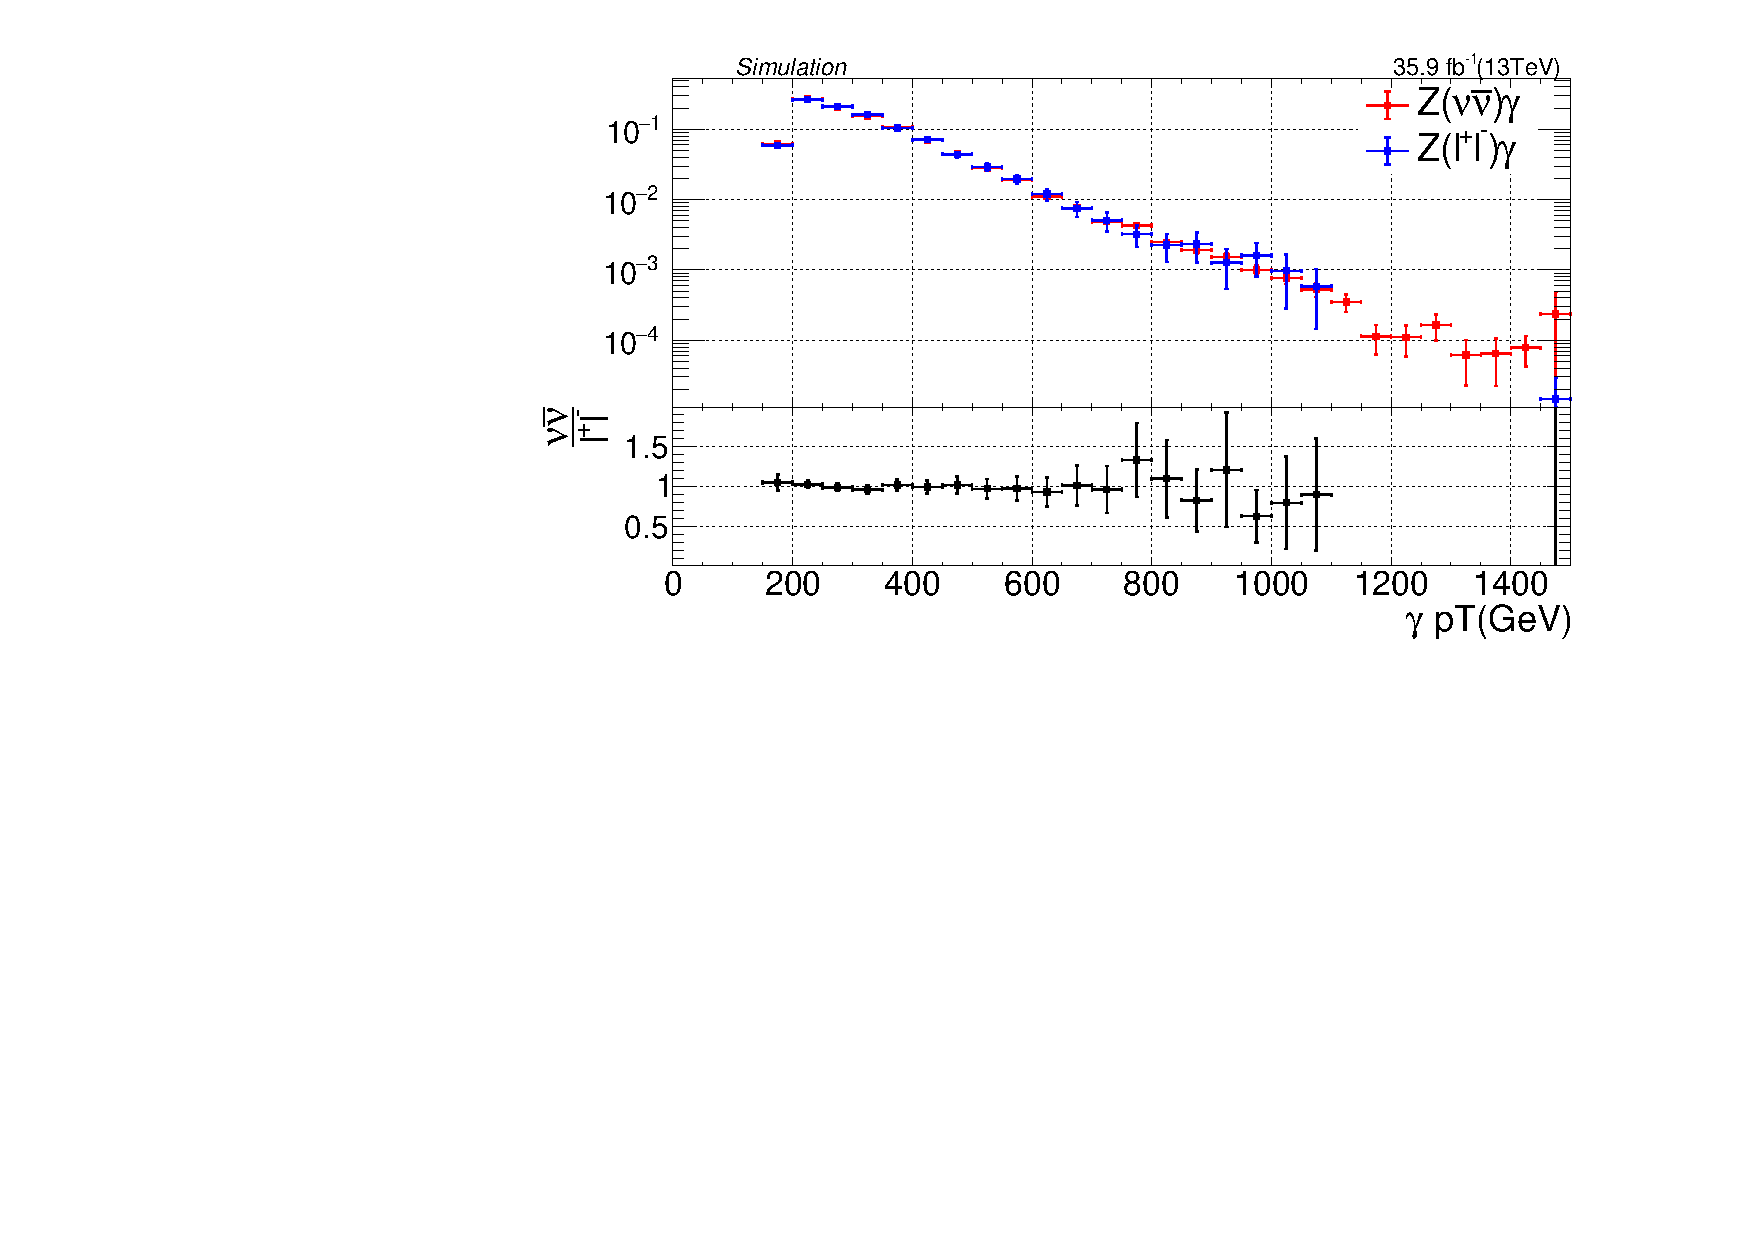
\includegraphics[width=0.48\linewidth]{../Figures/Chap3/zgamma/BestPhotonPtNuNu_LL_LO.pdf}
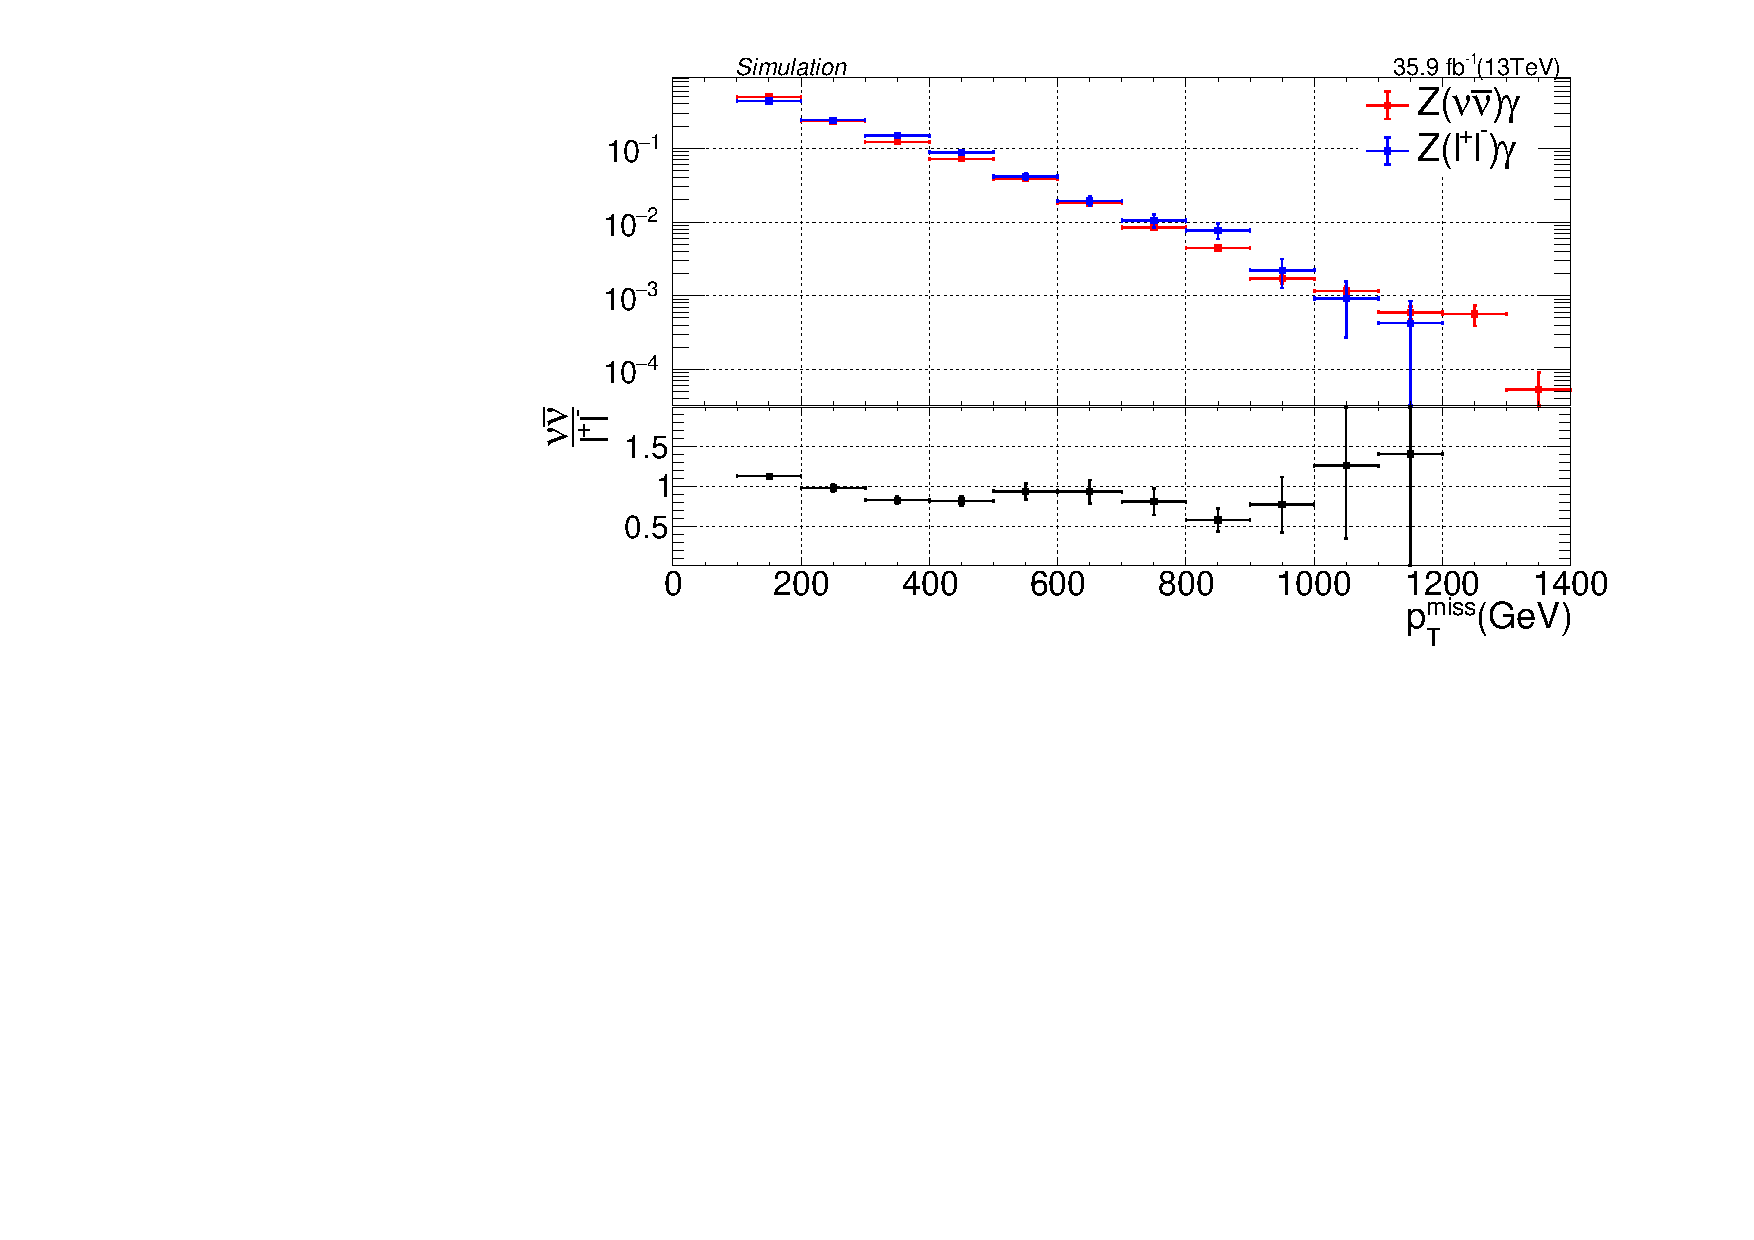
\includegraphics[width=0.48\linewidth]{../Figures/Chap3/zgamma/METNuNu_LL_LO.pdf}\\
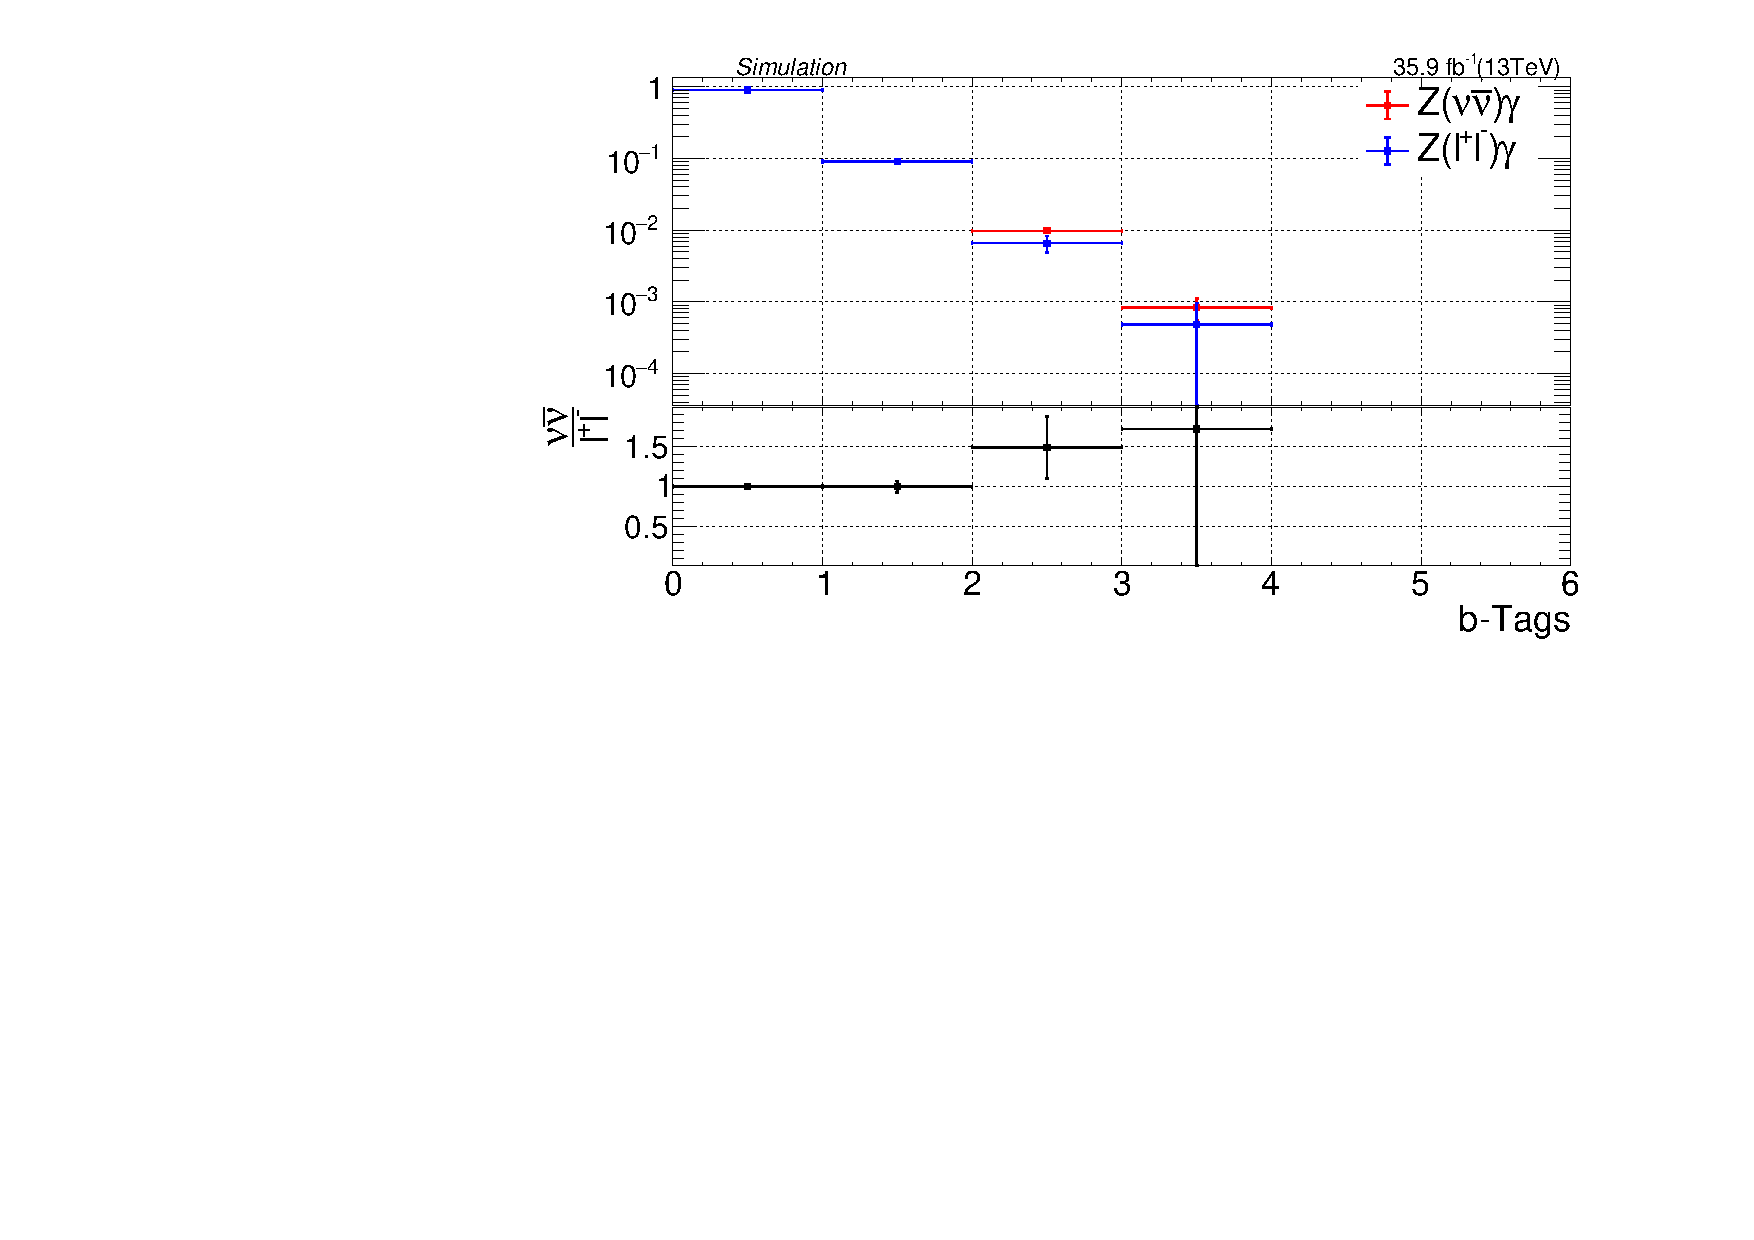
\includegraphics[width=0.48\linewidth]{../Figures/Chap3/zgamma/nBTagsNuNu_LL_LO.pdf}
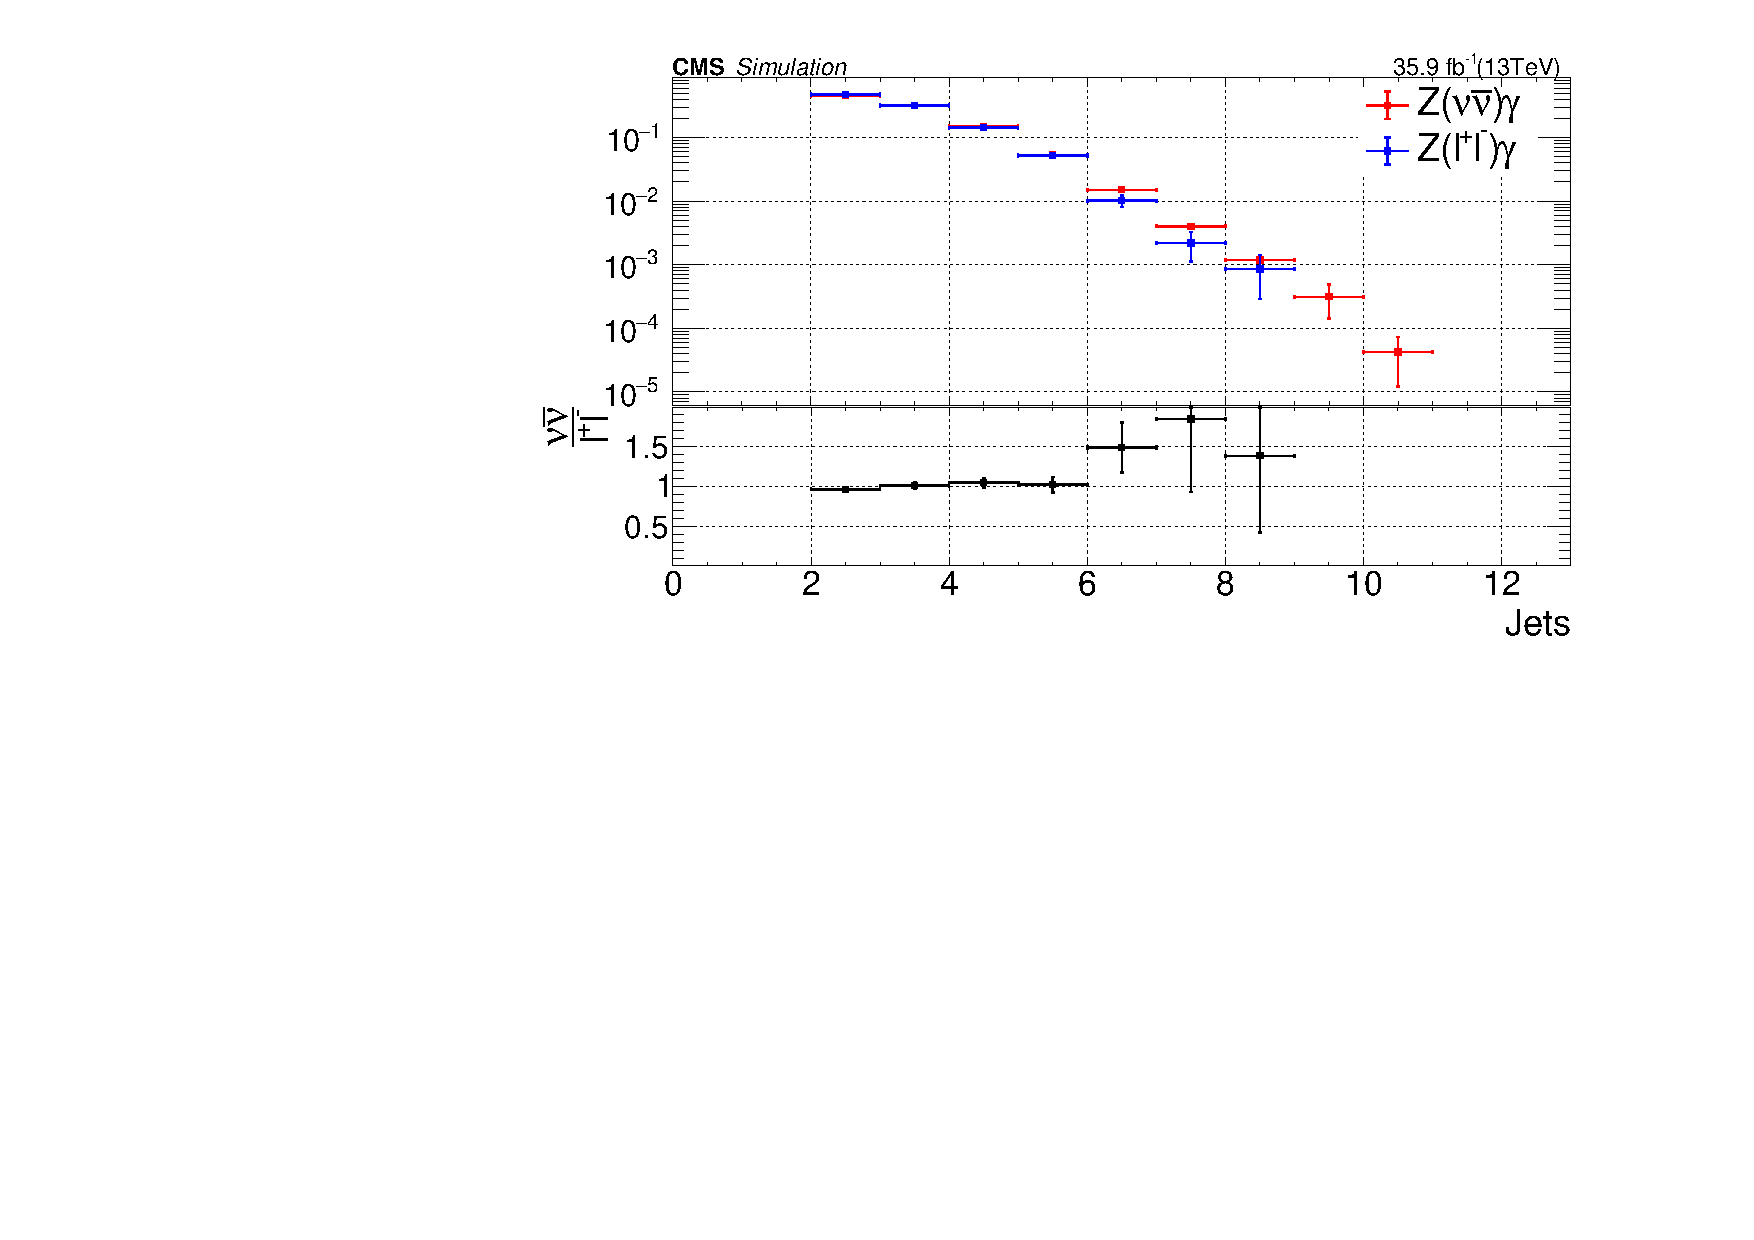
\includegraphics[width=0.48\linewidth]{../Figures/Chap3/zgamma/nHadJetsNuNu_LL_LO.pdf}
\caption[Comparing $Z(ll)\gamma$ with $Z(\nu\nu)\gamma$]{Comparison of $Z(ll)\gamma$ with $Z(\nu\nu)\gamma$ as function of \ptg (top left), \ptmiss (top right), \nb (bottom left) and \nj (bottom right) for $\ptg>190\ \gev$}
\label{fig:ZGTF}
\end{figure}

The purity of the Z($\ell\ell$)+$\gamma$ control region is determined from a fit 
to the invariant mass, $m_{\ell\ell}$, distribution.  This isolates contamination 
from $\gamma t\bar{t}$ events, which are expected to have a roughly flat distribution.
The purity is checked in three different ways, using MC to predict the number of 
$t\bar{t}\gamma$ events, using a fit to the $m_{\ell\ell}$ distribution, and
using the opposite-sign, different-flavor control sample ($e\mu\gamma$).  All three
prediction give consistent results when calculated within the baseline phase-space, 
which are reported in Table~\ref{tab:zGammaPurity}. 
%Figure~\ref{fig:DYgammaPurity} 
%shows the observed $m_{\ell\ell}$ distribution plus the fitted mass spectrum. 
The uncertainties associated with our prediction of the 
$Z(\ell\ell)\gamma$ purity is also propagated to the final 
$Z\gamma$ prediction. 

%\begin{figure}
%\centering
%\includegraphics[width=0.48\linewidth]{../Figures/Chap3/zgamma/ZgammaPurityFit.png}
%\caption{Distribution of $m_{\ell\ell}$ for data and MC.  All events shown are required
%to pass the DY-$\gamma$ selections.}
%\label{fig:DYgammaPurity}
%\end{figure}

\begin{table}[h!]
\centering
\caption{Purity in the $Z\gamma$ control region.}
\label{tab:zGammaPurity}
\begin{tabular}{c|c|c|c}
\hline
         & \multicolumn{3}{c}{Method} \\\cline{2-4}
\nb      & MC              & $m_{\ell\ell}$ fits & $e\mu$ CR \\\hline\hline
%$=0$     & 0.995 $\pm$ 0.005  & -    & 0.968 $\pm$ 0.032  & 0.99 $\pm$ 0.01 \\\hline
%$\geq 1$ & 0.844 $\pm$ 0.065  & -    & 1.0   $\pm$ 0.0    & 0.84 $\pm$ 0.16 \\ \hline  
$\geq 0$ & 0.978 $\pm$ 0.009  & 0.97 & 0.97 $\pm$ 0.03   \\\hline
\end{tabular}
\end{table}

Because of the very low statistics in low \dphi region in data, we make use of scale factors that are derived using high \dphi events to predict events in the low \dphi region. Scale factor is given by eqn.\ref{eqn:ZGSF} and it is found to be $1.11\pm0.21$.
\begin{equation}
\label{eqn:ZGSF}
SF = \bigg(\frac{N_{ll+\gamma}^{data}\cdot \beta_{ll+\gamma}}{N^{\text{MC}}_{\nu\nu+\gamma}}\bigg)^{p^T_\gamma > 190,high\ \dphi}
\end{equation}
Prediction in low \dphi region is,
\begin{equation}
N_{\nu\nu+\gamma}^{data}(SR\ Bin) = SF\cdot N^{\text{MC}}_{\nu\nu+\gamma}(SR\ Bin)
\end{equation}
%For 0 b-tag SF is $1.10\pm0.22$ and for $\geq$ 1 b-tag region SF is $1.38\pm0.72$.

To account for systematic uncertainties associated with the MC
modeling of the \ptmiss shape, we apply the full electro-weak corrections obtained from 
theory calculations \cite{Denner:2015fca} as a function of \ptmiss. These uncertainties are listed in Table \ref{tab:EWcorr}.
they can be as high as 40\% in highest \ptmiss bin. These uncertainties are treated as
correlated across \ptmiss bins for the limit setting procedure. Uncertainties from b-tag SF are also considered and they are 2\% in 0b-tag bins and 6\% in $\geq1$b-tag bins. The b-tag SF uncertainty is treated as anti-correlated in 0 and $\geq1$ b-tag bins. Final predictions for Z$(\nu\nu)+\gamma$ are listed in Table \ref{tab:znnPredictions} for high \dphi and in Table \ref{tab:znnLDPPredictions} for low \dphi regions.

\begin{table}[h!]
\centering
\caption{Electroweak corrections as a function of \ptmiss.}
\label{tab:EWcorr}
\begin{tabular}{|c|c|}
\hline  \ptmiss~(GeV) & \% EW Correction  \\ 
\hline  100-200 &  8\\ 
\hline  200-270 &  18\\ 
\hline  270-350 &  20\\ 
\hline  350-450 &  25\\ 
\hline  450-750 &  35\\ 
\hline  $\geq$ 750&  40\\ 
\hline 
\end{tabular}
\end{table} 
